\section{Auswertung}
\label{sec:Auswertung}

\subsection{Filterkurve und Bestimmung der Güte}
\label{sec:Filterkurve und Bestimmung der Güte}

Im ersten Versuchsteil sollte die Güte des Selektivverstärkers untersucht werden. Dazu
wurde zu verschiedenen Eingangsfrequenzen bei konstanter Amplitude die Ausgangsspannung
vom Filter gemessen. Die dabei aufgenommenen Daten sind in \autoref{tab:filterkurve}
abgedruckt.

\begin{table}
  \centering
  \caption{Messdaten zur Bestimmung der Filterkurve.}
  \label{tab:filterkurve}
  \sisetup{table-format=2.1}
  \begin{tabular}{c c}
  \toprule
  $f / \si{kHz}$	& $U / \si{V}$ \\
  \midrule
  18,9&0,08	\\
  20,2&0,09	\\
  22,1&0,12	\\
  23,0&0,14	\\
  27,2&0,205	\\
  29,0&0,26	\\
  31,0&0,44	\\
  32,4&0,5	\\
  33,7&0,42	\\
  33,9&0,51	\\
  34,0&0,5	\\
  34,3&0,55	\\
  35,7&0,66	\\
  36,0&0,64	\\
  36,8&0,54	\\
  37,1&0,49	\\
  39,1&0,28	\\
  41,0&0,19	\\
  42,7&0,16	\\
  42,9&0,33	\\
  46,5&0,14	\\
  52,3&0,09	\\
  \bottomrule
  \end{tabular}
\end{table}
Die Güte ist, wie in \autoref{sec:Theorie} schon erwähnt, die relative Breite der Kurve
\[
	Q = \frac{\nu_0}{\nu_+ - \nu_-}.
\]
Für die Berechnung der Güte wird in einer nicht linearen Ausgleichsrechnung eine
Gaußglocke
\begin{equation}
	\label{eqn:gauss-glocke}
	f(\nu) = N * \exp\left(-a \cdot (\nu - \mu)^2\right)
\end{equation}
an die Messdaten gefittet.
\\
Wegen
\begin{equation}
	f(\nu_+) \overset{!}{=} 
	f(\nu_-) \overset{!}{=} 
	\frac{f(\mu)}{\sqrt{2}}
\end{equation}
folgt dann
\begin{equation}
	\label{eqn:nu-plus-minus}
	\nu_\pm = \mu \pm \sqrt{\frac{1}{2a} \ln(2)}
\end{equation}
und 
\begin{equation}
	\label{eqn:Q-Auswertung}
	Q = \frac{\mu}{\sqrt{2/a \ln(2)}}.
\end{equation}

Die nicht lineare Ausgleichsrechnung ergab die Fitparameter
\begin{align}
	\label{eqn:fit-ergebnisse}
	\mu &= (34,8 \pm 0,5) \si{kHz}, \\
	a &= (0,0139 \pm 0,0025) \si{s}, \\
	n &= (0,53 \pm 0,028) \si{V}.
\end{align}

Mit \autoref{eqn:Q-Auswertung} folgt dann unter Verwendung linearer Fehlerfortpflanzung
\begin{equation}
	Q = 3,48 \pm 0,5.
\end{equation}

Die Messdaten und die Ausgleichsfunktion sind in \autoref{fig:filterkurve} dargestellt.

\begin{figure}
	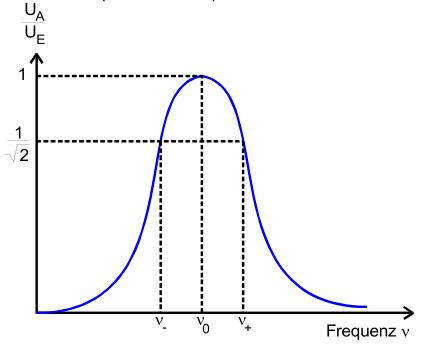
\includegraphics{build/filterkurve.pdf}
	\caption{Plot der Messdaten, der Ausgleichsfunktion sowie der Filterkurve die bei
	$Q=50$ zu erwarten wäre.}
	\label{fig:filterkurve}
\end{figure}

\subsection{Berechnung der Suszeptibilitäten}
\label{sec:Berechnung der Suszeptibilitäten}

In \autoref{sec:Theorie} wurde eine Formel für die Suszeptibilitäten hergeleitet. Die
Rechnung wird hier am Beispiel des $\symup{Gd_2O_3}$ einmal gezeigt. Die
Elektronenkonfiguration von $\symup{Gd}$ besteht abgesehen vom Xe-Teil aus sieben 4f-,
einem 5d- und zwei 6s-Elektronen.
Laut Versuchsanleitung hat $\symup{Gd^{3+}}$ sieben 4f-Elektronen, damit fehlen die 5d-
und 6s-Elektronen. Die sieben Elektronen richten ihre Spins nach der ersten Hundschen Regel gleich
aus, woraus sich der Gesamtspin
\[
	S = 7 \cdot \frac 12 = 3,5
\]
zusammensetzt. Da sich die Elektronen in der f-Schale aufhalten, ist
$\mathcal{l}_\text{max} = 3$. Der Bahndrehimpuls ist damit
\[
	L = -3 -2 -1 + 0 + 1 + 2 + 3 = 0.
\]
Weil mehr als halb voll ist folgt dann $J = L + S = 3,5$. Der Landé-Faktor für
$\symup{Gd^{3+}}$ ist damit
\[
	g_J(\symup{Gd^{3+}}) = 2.
\]
Die Teilchendichte ergibt sich gemäß
\[
	N = \frac{\rho}{M} N_A
\]
mit der dichte $\rho$, der molaren Masse $M$ und der Avogradokonstanten $N_A$.
\\
$N$ und $g_J$ können nun in die Gleichung für $\chi$ eingesetzt werden, die Ergebnisse
sind in \autoref{tab:theo-susz} zusammengefasst.
\begin{table}
  \centering
  \caption{Kennwerte und errechnete Suszeptibilitäten zu den untersuchten Stoffen.}
  \label{tab:theo-susz}
  \sisetup{table-format=2.1}
  \begin{tabular}{c c c}
  \toprule
   & $\symup{Gd_2O_3}$ 	& $\symup{Dy_2O_3}$\\
  \midrule
  % content
  4f-Elektronen                           & 7      & 9      \\
L                                         & 0      & 5      \\
S                                         & 3,5    & 2,5    \\
J                                         & 3,5    & 7,5    \\
$g_J$                                     & 2,0    & 1,33   \\
$\rho \, / \, \si{\kilo\gram\per\meter³}$ & 7400   & 7800   \\
$m \, / \, \si{\kilo\gram}$               & 0,0141 & 0,0151 \\
$M/\si{\gram\per\mol}$           	  & 362   & 373   \\
$N \cdot \num{e28}/\si{\meter³}$ 	  & 2,46  & 2,52  \\
$\chi_\text{theo}$               	  & 0,014 & 0,026 \\
  \bottomrule
  \end{tabular}
\end{table}

\subsection{Experimentelle Bestimmung der Suszeptibilitäten}
\label{sec:Experimentelle Bestimmung der Suszeptibilitäten}

Bestimmung wurde im Experiment mit einer Brückenschaltung gearbeitet. Die Speisespannung
hatte eine Amplitude von $U_\text{Sp} = \SI{0.9}{\volt}$.

\subsubsection{$\symup{Dy_2O_3}$}
\label{sec:ausw-Dy2O3}

Vor der Messung wurde die Brücke abgeglichen auf $R_3 = \SI{1001.2}{\ohm}$ mit einer
Restspannung an der Brücke von $U_\text{Br} = \SI{12.5}{m\volt}$. Danach wurde in drei
Durchläufen die Probe in eine Spule eingesetzt. Die Brückenspannung nach Einschieben, der
zum erneuten Abgleichen notwendige Widerstand $R_3^\prime$ sowie die Differenz 
$\Delta R = R_3 - R_3^\prime$ sind in \autoref{tab:probe1} dargestellt.

\begin{table}
  \centering
  \caption{Messwerte zu $\symup{Dy_2O_3}$.}
  \label{tab:probe1}
  \sisetup{table-format=2.1}
  \begin{tabular}{c c c c c}
  \toprule
  Durchlauf &
  $U_\text{Br}^\prime / \si{m\volt}$ &
  $\Delta U_\text{Br} / \si{m\volt}$ &
  $R_3^\prime / \si{\ohm} $ &
  $\Delta R_3 / \si{\ohm} $ \\
  \midrule
  % content
  1 & 60 & 47,5 & 999,55 & 1,62 \\
  2 & 66 & 53,5 & 999,51 & 1,655 \\
  3 & 66 & 53,5 & 999,55 & 1,615 \\
  \bottomrule
  \end{tabular}
\end{table}
\noindent
Aus den Formeln für Mittelwert und Standartabweichung folgen
\begin{equation}
	\Delta R = (1,63 \pm 0,018) \,\symup\Omega
	\qquad
	U_\text{Br} = (64 \pm 2,8) \,\symup{mV}
\end{equation}
Mit der gemessenen Länge der Probe
$L = \SI{0.173}{\meter}$ folgt mit der Dichte und Masse der Probe 
(vgl. \autoref{tab:theo-susz}) der Probenquerschnitt 
\[
	Q =  \frac{m_\text{Pr}}{L \cdot \rho_\text{w}}
	= 2,85 \cdot 10^{-5} \,\symup{m}^2
\]
Mit den zwei Methoden für die Bestimmung der Suszeptibilität folgen dann zwei Ergebnisse
für $\chi(\symup{Dy_2O_3})$:
\begin{equation}
	\chi_U = 0,069 \pm 0,004
	\qquad
	\chi_R = 0,00987 \pm 0,00011
\end{equation}
Die Spannungsdifferenz wurde im auswertenden Programm um eine Zehnerpotenz runterskaliert, da
im Filter ein zehnfach-Gain aktiviert wurde. Für die Messungenauigkeit wurde 
mit linearer Fehlerfortpflanzung gerechnet.

\subsubsection{$\symup{Gd_2O_3}$}

Das Vorgehen erfolgte analog zu dem in \autoref{sec:ausw-Dy2O3} Beschriebenen. Die Brücke
wurde immer zu Beginn auf $R_3 = \SI{1001.065}{\ohm}$ mit $U_\text{Br} =
\SI{12.5}{m\volt}$ abgeglichen. Die Messwerte sind in \autoref{tab:probe3} dargestellt.

\begin{table}
  \centering
  \caption{Messwerte zu $\symup{Gd_2O_3}$.}
  \label{tab:probe3}
  \sisetup{table-format=2.1}
  \begin{tabular}{c c c c c}
  \toprule
  Durchlauf &
  $U_\text{Br}^\prime / \si{m\volt}$ &
  $\Delta U_\text{Br} / \si{m\volt}$ &
  $R_3^\prime / \si{\ohm} $ &
  $\Delta R_3 / \si{\ohm} $ \\
  \midrule
  % content
  1 & 31 & 18,5 & 1000,37 & 0,695 \\
  2 & 33 & 20,5 & 1000,31 & 0,755 \\
  3 & 30.5 & 18 & 1000,31 & 0,755 \\
  \bottomrule
  \end{tabular}
\end{table}

Wie beim Dysprosiumoxid kann auch hier mit den Formeln für Mittelwert und
Standartabweichung gearbeitet werden, damit folgen 
\begin{equation}
	\Delta U_\text{Br} = (31,5 \pm 1,1) \symup{mV}
	\quad
	\text{und}
	\quad
	\Delta R_3 = (0,735 \pm 0,028) \symup\Omega.
\end{equation}

Mit der gemessenen Länge $L = \SI{0.176}{\meter}$ folgt mit den Werten für Masse und Dichte
die Querschnittsfläche der Probe
\begin{equation}
	Q = 2,503 \cdot 10^{-5} \symup{m}^2.
\end{equation}

Abschließend können dann zwei Werte für $\chi(\symup{Gd_2O_3})$ bestimmt werden:
\begin{equation}
	\chi_\text{U} = 0,0292 \pm 0,0017
	\quad
	\chi_\text{R} = 0,00508 \pm 0,0002
\end{equation}
Wie bei $\chi(\symup{Dy_2O_3})$ musste auch hier $\Delta U_\text{Br}$ um Zehnfaches
runterskaliert werden.

